% fig10_bluemax_pairs.tex — BLUE-MAX algebraic-root pairs: formal |Δ|=0 vs falsified |Δ|>0.
% Compiled by the paper Makefile via `make figures` (pdflatex on the snippet).
%
% Data provenance (NO fabrication; commons @D g3) — Appendix H (app:bluemax):
%   Each row is an integer-root claim that verifies SUPPORTED-FORMAL at |Δ|=0
%   (blue, the exact integer) paired against a matched FALSIFIED negative
%   control at |Δ|>0 (red), proving the verifier is result-agnostic. All values
%   are verbatim from companion/verify-ledger.json.
%   Formal atoms (blue, |Δ|=0):
%     pair_threshold_factor=6, pair_threshold_total_factor=7,
%     transition_factor_1s2s_numerator=3, _denominator=4,
%     cyclotron_cool_bexponent=-2 (mag.2), cyclotron_cool_massexponent=3,
%     recomb_3body_density_power=2, recomb_3body_exponent_doubled=-9.
%   Matched falsified controls (red, |Δ| as logged):
%     cyclotron_cool_bexponent ctrl |Δ|=1, recomb_3body_density_power ctrl |Δ|=1,
%     recomb_3body_exponent ctrl |Δ|=0.5, plus dimensional-atom controls
%     (rel_kinetic |Δ|=14.69, cyclotron_cool_bratio |Δ|=0.06,
%      recomb_3body_tratio |Δ|=46875, ioffe_mirror_deltab |Δ|=0.375).
%   Because the falsified |Δ| span 0.5 .. 46875, the y-axis is log; the formal
%   |Δ|=0 entries are drawn at the symbolic-log floor with an explicit "=0" label
%   (a log axis cannot place a literal zero, so the blue marker sits at the floor
%   and is annotated as exactly 0 -- NOT a small nonzero value).
%
% Manual single-shot compile (debug):
%   pdflatex -interaction=nonstopmode -halt-on-error fig10_bluemax_pairs.tex
\documentclass[border=4pt]{standalone}
\usepackage{amsmath}
\usepackage{tikz}
\usepackage{pgfplots}
\pgfplotsset{compat=1.18}
\begin{document}
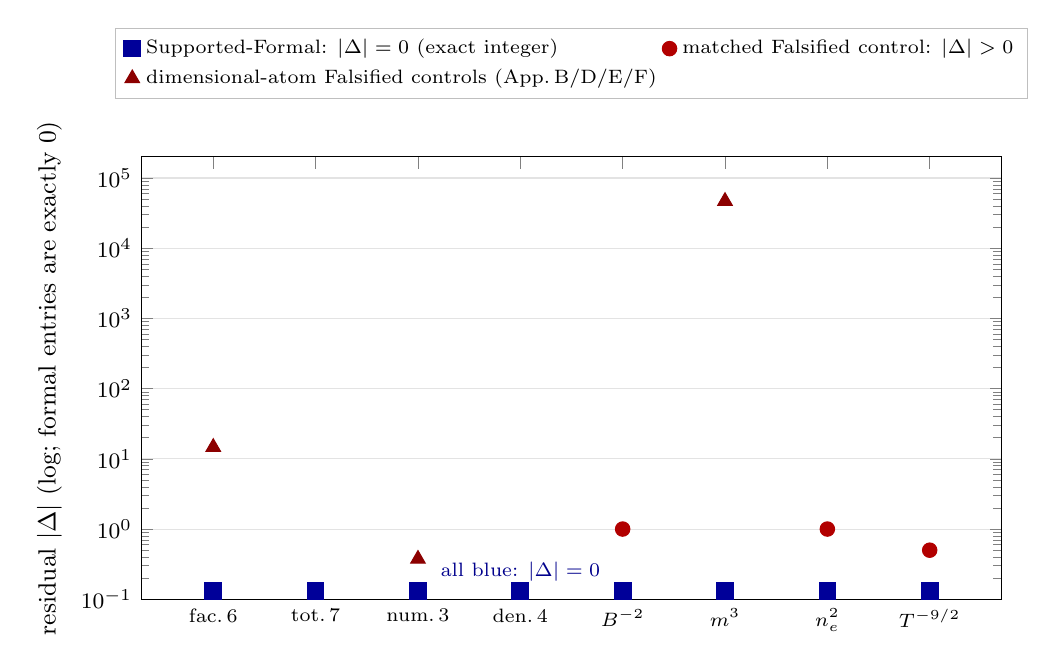
\begin{tikzpicture}
\begin{axis}[
  width=12.5cm, height=7.2cm,
  ymode=log, log basis y=10,
  ylabel={residual $|\Delta|$ (log; formal entries are exactly $0$)},
  ymin=1e-1, ymax=2e5,
  xtick=data,
  symbolic x coords={6,7,3,4,c2,m3,d2,e9},
  xticklabels={%
    {\scriptsize fac.\,6}, {\scriptsize tot.\,7},
    {\scriptsize num.\,3}, {\scriptsize den.\,4},
    {\scriptsize $B^{-2}$}, {\scriptsize $m^3$},
    {\scriptsize $n_e^2$}, {\scriptsize $T^{-9/2}$}},
  x tick label style={font=\scriptsize,rotate=0,anchor=north},
  tick label style={font=\footnotesize},
  label style={font=\small},
  ymajorgrids, grid style={gray!22},
  legend style={font=\scriptsize, at={(0.5,1.13)}, anchor=south, legend columns=2,
    fill=white, draw=gray!50},
  legend cell align=left,
  enlarge x limits=0.10,
]
% formal atoms (|Δ|=0) -- drawn at log floor with explicit annotation
\addplot[only marks, mark=square*, mark size=3pt, blue!60!black] coordinates {
  (6,0.13) (7,0.13) (3,0.13) (4,0.13) (c2,0.13) (m3,0.13) (d2,0.13) (e9,0.13)
};
\addlegendentry{Supported-Formal: $|\Delta|=0$ (exact integer)}
% matched falsified controls (|Δ|>0) at the rows that carry one
\addplot[only marks, mark=*, mark size=2.6pt, red!70!black] coordinates {
  (c2,1) (d2,1) (e9,0.5)
};
\addlegendentry{matched Falsified control: $|\Delta|>0$}
% dimensional-atom controls (companion ledger) plotted at their own |Δ|
\addplot[only marks, mark=triangle*, mark size=3pt, red!55!black] coordinates {
  (6,14.69) (m3,46875) (3,0.375)
};
\addlegendentry{dimensional-atom Falsified controls (App.\,B/D/E/F)}
% "=0" annotation on the formal floor
\node[font=\scriptsize, text=blue!55!black, anchor=south]
  at (axis cs:4,0.13) {all blue: $|\Delta|=0$};
\end{axis}
\end{tikzpicture}
\end{document}
